\documentclass{article}
%----------------------------------------------------------------------------------------
%	PACKAGES AND OTHER DOCUMENT CONFIGURATIONS
%----------------------------------------------------------------------------------------
\usepackage[utf8]{inputenc}% gestion des accents (source)
\usepackage[T1]{fontenc}% gestion des accents (PDF)
\usepackage[francais]{babel}% gestion du français
\usepackage{natbib}% utilisation du lib de référence zotero
\usepackage{textcomp}% caractères additionnels
\usepackage{mathtools,amssymb,amsthm}% packages de l'AMS + mathtools
\usepackage{lmodern}% police de caractère
\usepackage{geometry}% gestion des marges
\usepackage{graphicx}% gestion des images
\usepackage{caption}% gestion des figures
\usepackage{subcaption}% sous figures
\usepackage{xcolor}% gestion des couleurs
\usepackage{array}% gestion améliorée des tableaux
\usepackage{calc}% syntaxe naurelle pour les calculs
\usepackage{titlesec}% pour les sections
\usepackage{titletoc}% pour la table des matières
\usepackage{fancyhdr}% pour les en-têtes
\usepackage{titling}% pour le titre
\usepackage{enumitem}% pour les listes numérotées
\usepackage[hyphens]{url} % Pour des césures correctes dansles URLs
\usepackage{pythonhighlight}
\usepackage{hyperref}
\usepackage{titlesec}
\usepackage{csquotes} % Context sensitive quotation facilities
\usepackage[yyyymmdd]{datetime} % Uses YEAR-MONTH-DAY format for dates
% Taille des marges
\geometry{hmargin=2cm,vmargin=2.8cm}
\renewcommand{\dateseparator}{-} % Sets dateseparator to '-'
% RAZ des numéros de section après un chapitre
\makeatletter\@addtoreset{section}{chapter}\makeatother
% Pour mettre des I, II, etc. aux parties
\renewcommand{\thepart}{\Roman{part}}
% Pour mettre des 1, 2, etc. aux chapitres
\renewcommand{\thechapter}{\Roman{chapter}}
% Idem pour les sections et avoir le numéro de chapitre
\renewcommand{\thesection}{\Roman{section}}
% Idem pour les sous-sections et avoir le numéro de chapitre
\renewcommand{\thesubsection}{\Roman{section}.\arabic{subsection}}

\usepackage{fancyhdr} % Headers and footers
\pagestyle{fancy} % All pages have headers and footers
\fancyhead[R]{Prédiction des retards de trains}
\fancyfoot[C]{\thepage} % Custom footer text
\fancyfoot[R]{2023-2024} % Custom footer text
\newcommand{\note}[1]{\marginpar{\scriptsize \textcolor{red}{#1}}} % Enables comments in red on margin

\renewcommand{\thefigure}{\arabic{section}.\arabic{figure}}
\makeatletter
\@addtoreset{figure}{section}
% annexe
\usepackage[toc,page,title,titletoc,header]{appendix} % pour les annexes
\renewcommand{\appendixtocname}{Table des annexes} % indique le nom de la table des annexes dans la toc
\renewcommand{\appendixpagename}{Annexes} % Nom du titre de la page des annexes
\usepackage{etoolbox}
\AtBeginEnvironment{appendices}{\renewcommand{\thesection}{\Alph{section}}}


%Matlab code

\usepackage[utf8]{inputenc}

\usepackage{listings}
\usepackage{xcolor}

\definecolor{codegreen}{rgb}{0,0.6,0}
\definecolor{codegray}{rgb}{0.5,0.5,0.5}
\definecolor{codepurple}{rgb}{0.58,0,0.82}
\definecolor{backcolour}{rgb}{0.95,0.95,0.92}

\lstdefinestyle{mystyle}{
    backgroundcolor=\color{backcolour},   
    commentstyle=\color{codegreen},
    keywordstyle=\color{blue},
    numberstyle=\tiny\color{codegray},
    stringstyle=\color{codepurple},
    basicstyle=\ttfamily\footnotesize,
    breakatwhitespace=false,         
    breaklines=true,                 
    captionpos=b,                    
    keepspaces=true,                 
    numbers=left,                    
    numbersep=5pt,                  
    showspaces=false,                
    showstringspaces=false,
    showtabs=false,                  
    tabsize=2
}

\lstset{style=mystyle}
\usepackage{float}
\usepackage[usenames,dvipsnames]{color}
\usepackage{tikz,forest}
\usetikzlibrary{arrows.meta}

\usepackage{multicol}

%----------------------------------------------------------------------------------------

\begin{document}

\begin{titlepage}
        \newcommand{\HRule}{\rule{\linewidth}{0.5mm}}
        \begin{center}
            % En-têtes
            \textsc{\LARGE{} Apprentissage automatique} \\[0.5cm] 
            \textsc{\Large{} CentraleSupélec - 3A} \\[0.5cm]
            % Titre
            \HRule \\[0.6cm]
            {\huge\bfseries{} Projet : prédiction des retards de trains} \\[0.25cm]
            \HRule \\[1.5cm]
            % Date
            {\large\today} \\[2cm] 
            % Logo CS
            \includegraphics[width=8cm]{LogoCS.png}
            \\[2cm] 
        \end{center}
        \vfill{}
        
        \begin{center}
        \Large{
            {Cindy Hua}\\
            {Rémi Boutonnier}\\
            {Romain Ageron}}
        \end{center} 
\end{titlepage}

   
    
% Table des matières
\tableofcontents

\newpage

\section{Introduction}

Nous nous plaçons dans le contexte où la SNCF souhaite évaluer un planning des trains (pour les 6 mois à venir par exemple). Nous considérons donc seulement les variables qui caractérisent les liaisons, et cherchons à prédire le retard à l'arrivée et ses causes.
\begin{multicols}{2}
Variables explicatives :
\begin{itemize}[label=\textbullet, itemsep=0pt, parsep=0pt]
    \item date
    \item service
    \item gare\_depart
    \item gare\_arrivee
    \item duree\_moyenne
    \item nb\_train\_prevu
    \item Longitude\_gare\_depart (ajoutée)
    \item Lattitude\_gare\_depart (ajoutée)
    \item Longitude\_gare\_arrivee (ajoutée)
    \item Lattitude\_gare\_arrivee (ajoutée)
    \item distance (ajoutée)
\end{itemize}
\columnbreak
Varaibles cibles :
\begin{itemize}[label=\textbullet, itemsep=0pt, parsep=0pt]
    \item retard\_moyen\_arrivee
    \item prct\_cause\_externe
    \item prct\_cause\_infra
    \item prct\_cause\_gestion\_trafic
    \item prct\_cause\_materiel\_roulant
    \item prct\_cause\_gestion\_gare
    \item prct\_cause\_prise\_en\_charge\_voyageurs
\end{itemize}
\end{multicols}


\bigskip
Cela ne laisse pas beaucoup de variables pour la prédiction, mais nous pourrions potentiellement utiliser d'autres données. Par exemple, la météo pourrait être liée au retard d'un train. Cependant, dans notre contexte cela n'est pas possible car il faudrait prédire la météo des 6 prochains mois.

\section{Analyse des données}

\subsection{Analyses}

\subsubsection{Analyse temporelle des variables}
Nous avons commencé par une analyse temporelle des variables d'entrée et de sortie:

\begin{figure}[H]
    \begin{subfigure}{0.3\textwidth}
        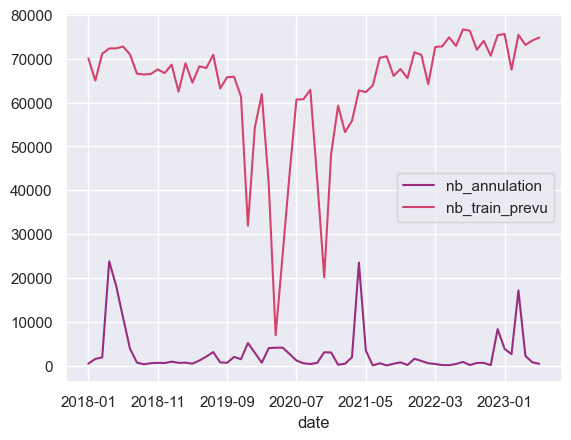
\includegraphics[width=\linewidth]{annules_prevus_tmp.png}
        \caption{Figure 1}
    \end{subfigure}
    \begin{subfigure}{0.3\textwidth}
        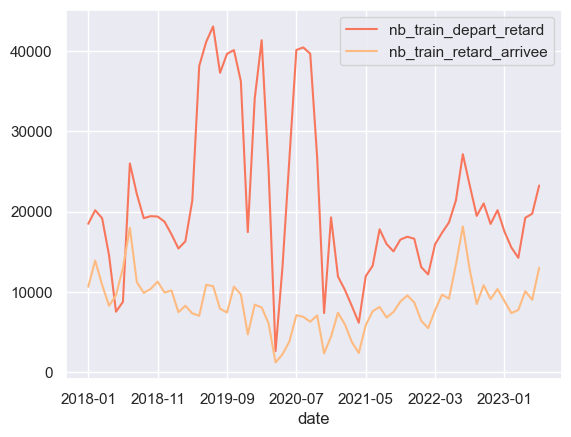
\includegraphics[width=\linewidth]{retard_tmp.png}
        \caption{Figure 2}
    \end{subfigure}
    \begin{subfigure}{0.3\textwidth}
        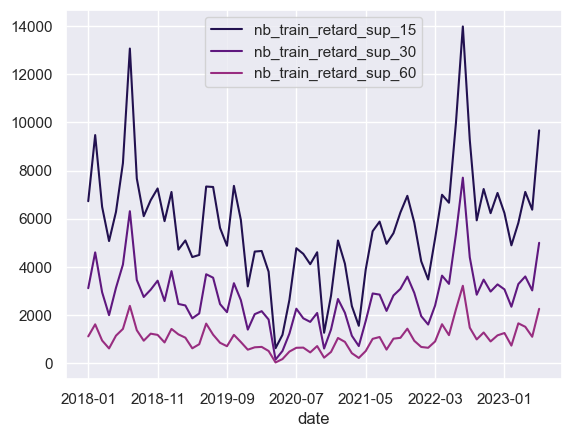
\includegraphics[width=\linewidth]{retard_cat_tmp.png}
        \caption{Figure 3}
    \end{subfigure}
    \caption{Analyse temporelle: de gauche à droite, évolution du nombre de trains prévus et annulés, du nombre de trains retardés, du nombre de trains retardés selon la catégorie de retard}
\end{figure}

On note notamment 3 pics du nombre de trains annulés en:
\begin{itemize}[label=\textbullet]
    \item avril et mai 2018: grève des cheminots
    \item avril 2021: période de confinement du 3 avril au 3 mai 2021
    \item mars 2023: grève contre la réforme des retraites
\end{itemize}

On remarque que le premier confinement n'a pas été si problématique pour les annulations de train car la SNCF avait déjà prévu moins de trains.

De même pour les retards de train, on note une grosse fluctuation autour du début de la période COVID, sans doute dû à un manque de personnels entrainant des contraintes à tous les niveaux. 


\subsubsection{Analyse de la répartition des variables}
Nous avons également étudié la répartition des variables en terme de proportion. En particulier, nous trouvons une répartition des retards moyens très semblables à une loi de Poisson: 
\begin{center}
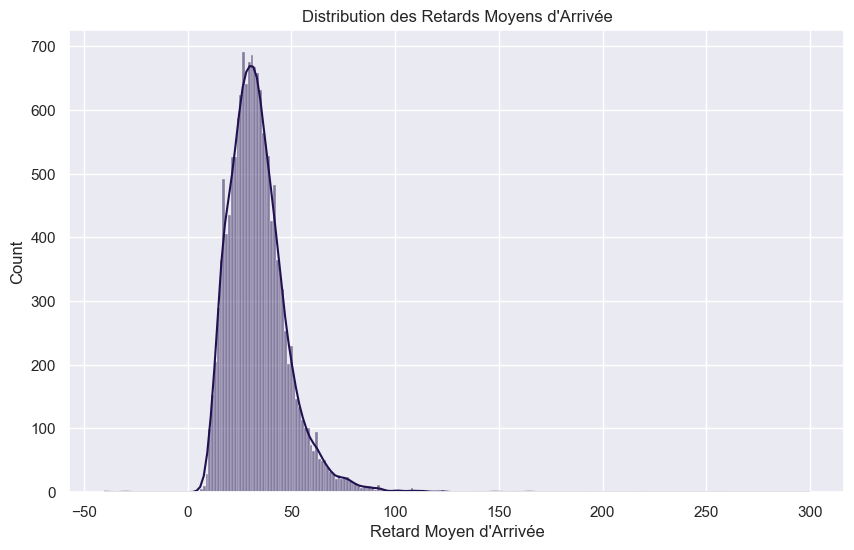
\includegraphics[width=10cm]{dist_retard_arrivee.png}
\end{center}

Nous pouvons aussi nous demander si les trajets longs sont plus amenés à rencontrer des retards:

\begin{center}
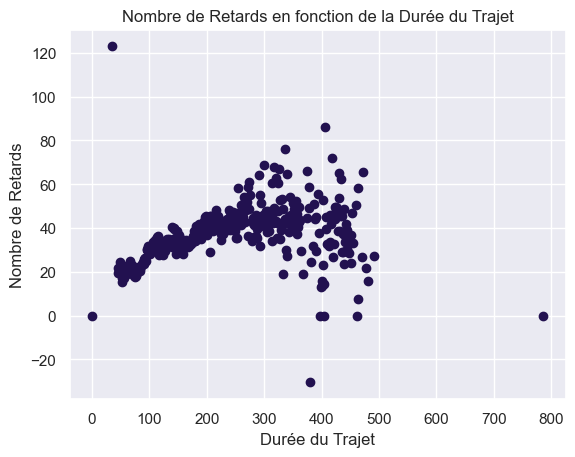
\includegraphics[width=10cm]{retard_ftn_duree.png}
\end{center}

Jusqu'à des trajets de 4 heures, il semblerait qu'on pourrait modéliser le nombre de retards en fonction de la durée de trajet comme une fonction linéaire. Pour des trajets plus longs, tout paraît possible: de très gros retards comme de l'avance. 

\subsubsection{Matrice de corrélation}
Nous avons voulu voir si certaines corrélations pouvaient être intéréssantes à discuter dans la grande matrice de corrélation: 

\begin{figure}[H]
    \centering
    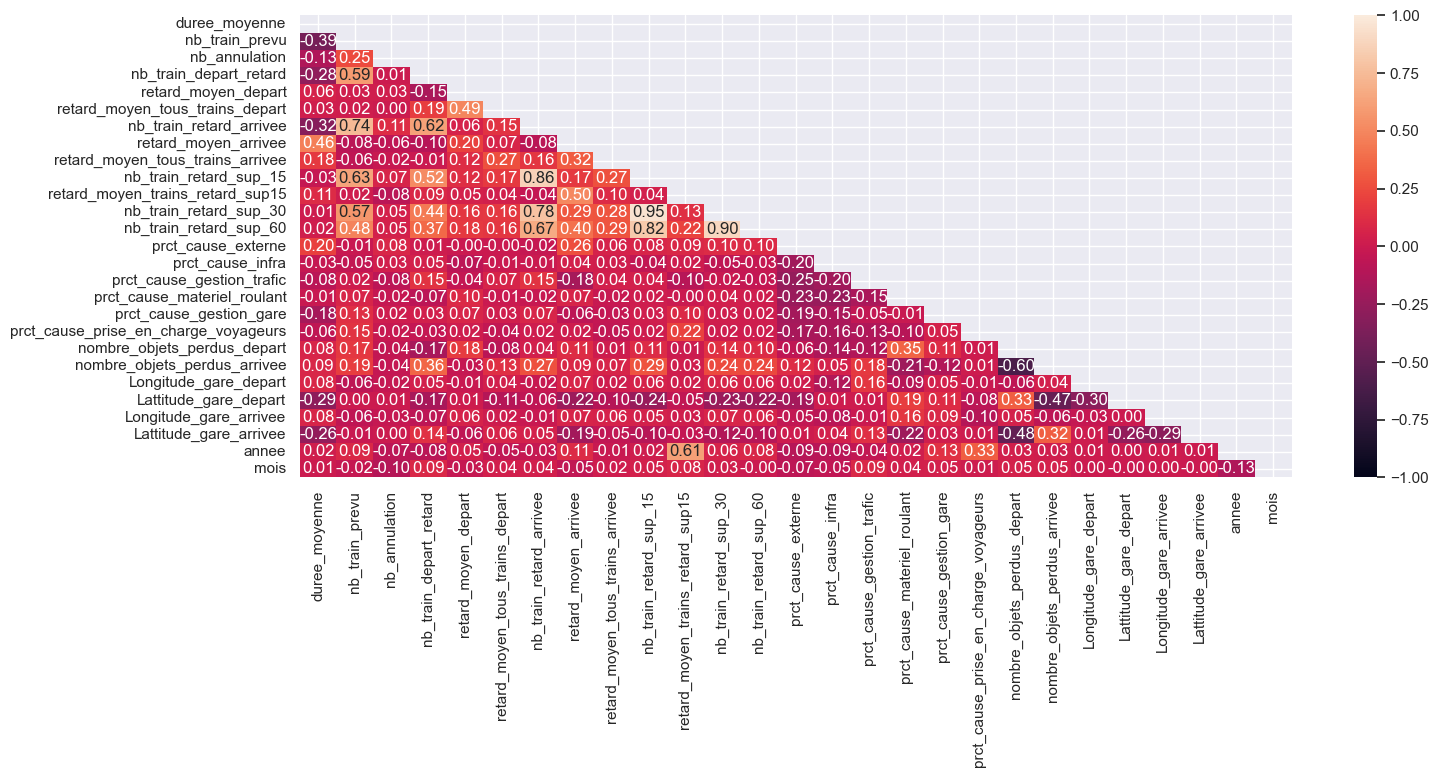
\includegraphics[scale=0.45]{corr_all.png}
    \caption{Matrice de corrélation de toutes les variables du dataset}
\end{figure}

Certaines grosses valeurs de corrélation sont prévisibles, par exemple celles reliant les différentes variables de retard. L'année est corrélée positivement au retard moyen puisque nous avons vu que l'année du COVID a été une année très importante pour les retards. 
D'autres relations ont été mise en avant comme la corrélation du retard moyen à l'arrivée et de la durée moyenne du trajet (corrélation de 0.46).

\subsection{Ajout de données}

Afin de compléter la base de données, nous avons cherché d'autres datasets sur le site de la SNCF: l'une contenant \href{https://ressources.data.sncf.com/explore/dataset/referentiel-gares-voyageurs/table/}{les coordonnées GPS de chacune des gares} , l'autre référençant l' \href{https://ressources.data.sncf.com/explore/dataset/objets-trouves-restitution/table/}{historique des objets perdus dans les gares}. La première nous permettra d'avoir la distance entre deux gares (en plus d'avoir déjà la durée moyenne entre les deux gares) tandis que la seconde permettra peut-être d'expliquer certaines causes de retard, notamment celles liées aux bagages abandonnés et au plan vigipirate. 


\subsection{Preprocessing}


\subsubsection{Features numériques}

Les pourcentages ont été normalisés entre 0 et 1. Les durées moyennes, nombres de trains prévus, distances et coordonnées GPS ont été centrés-réduits. La date était normalisée de manière affine pour avoir janvier 2018 = -1 et décembre 2022 = 1.

\subsubsection{Features catégorielles}

Les service, gare départ, gare d'arrivée et les mois ont été encodés par un one-hot encoding dans un premier temps puis de manière différente (voir \ref{sec:feat_eng}).

\subsubsection{Feature engineering}
\label{sec:feat_eng}

\paragraph{Ajout des mois:}

Même si l'information des mois est contenu dans la "partie décimale" de l'année, cela n'est pas vraiment accessible pour les modèles. Ajouter les mois avec un one-hot embedding donne accès facile à cette information pour les modèles. En pratique cela se traduit par une diminution de la rmse de 5\% à 10\% selon les modèles et les hyperparamètres. Cet embedding donne une séparation linéaire des différent mois (bien pour la régression linéaire par exemple) et est pratique pour les modèles basés sur des arbres de décisions (facile de faire une décision sur le mois).

L'un des problèmes avec cet embedding pour les KNNs est que tous les mois sont équidistants. Il semble pourtant raisonnable de supposer que le mois de Juillet est plus similaire au mois d'Août qu'au mois de Février. D'où l'embedding des mois sur un cercle : $f(mois) = \exp (i * mois * \pi / 6)$. Cela donne en pratique des résultats équivalents pour le KNN la plupart des autres méthodes, et des résultats nettement dégradés pour la régression linéaire (on ne peut plus prendre une contribution indépendante pour chaque mois). Un autre avantage est celui d'utiliser 2 dimensions au lieu de 12.


\paragraph{Importance des gares:}
Cette partie ne concerne que le KNN puisque les autres méthodes utilisées ne sont pas sensibles aux ordres de grandeurs relatifs des différentes features d'entrée. 

On peut supposer que pour deux liaisons avoir la même gare de départ et / ou d'arrivée peut avoir une forte influence sur les variables que l'ont souhaite prédire. Ainsi, dans le calcul de la distance dans le KNN, plutôt que de pénaliser la distance entre deux vecteurs par 0 si c'est la même liaison, 1 si c'est la même gare d'arrivée ou (exclusif) de départ, et 2 sinon, on peut utiliser un coefficient $\lambda$ de manière à accorder plus ou moins d'importance aux gares composant la liaison vis-à-vis des autres features afin de définir une meilleur notion de proximité pour le KNN. Plus généralement, on n'est pas obligé de se limiter à l'utilisation du même $\lambda$ pour la gare de départ ou d'arrivée. On va donc encoder les gares de départ par $\alpha \times one-hot$ et les gares d'arrivée par $\beta \times one-hot$. La figure \ref{erreur_a_b} montre l'erreur en fonction de ces paramètres.

\begin{figure}[H]
    \centering
    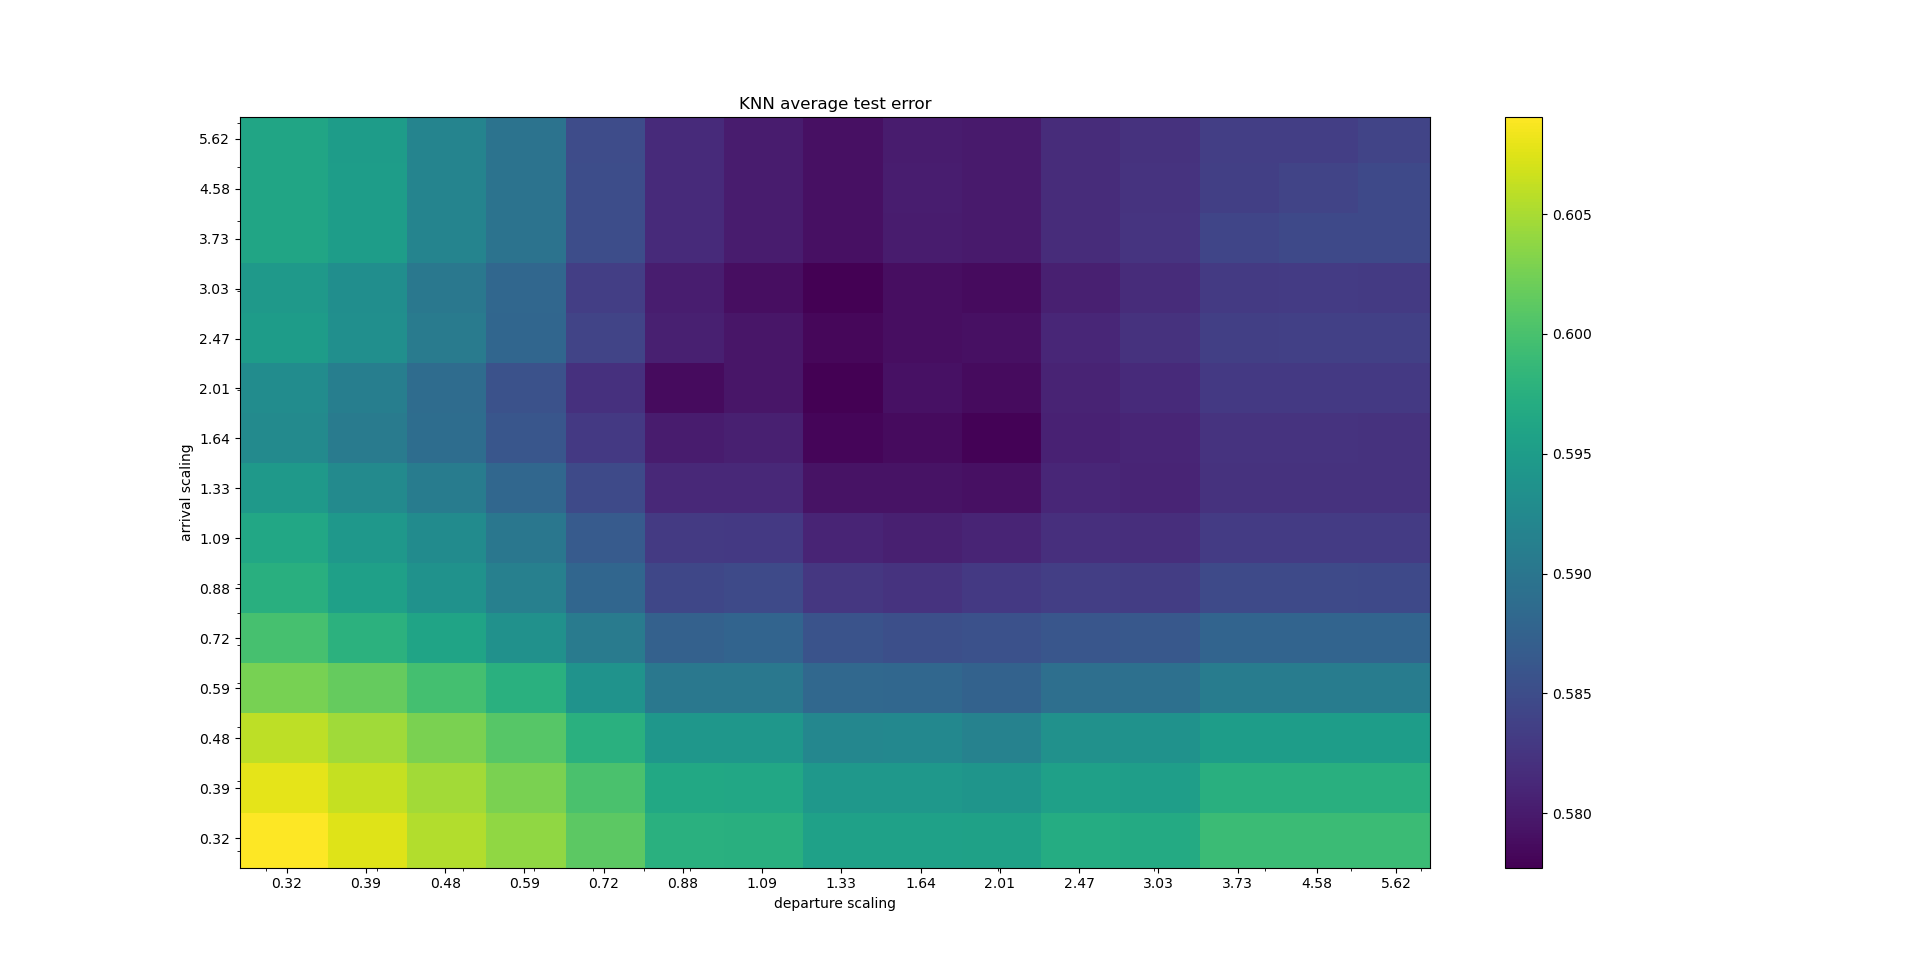
\includegraphics[scale=0.35]{station_scaling.png}
    \caption{Erreur moyenne de test selon $\alpha$ (abscisses) et $\beta$ (ordonnées)}
    \label{erreur_a_b}
\end{figure}

On observe qu'augmenter ces coefficients permet effectivement de diminuer l'erreur. Par ailleurs, on observe que la gare d'arrivée (coefficient plus élevé) semble avoir plus d'influence sur le résultat que la gare de départ. Les coefficients optimaux obtenus sont $\alpha = 4/3, \beta=2$. Cela permet une (faible) amélioration, diminuant la rmse moyenne d'environ 2\%.

\paragraph{Similarité des liaisons:}

L'attribution d'un coefficient différent pour les gares d'arrivée et de départ est en fait une manière de définir une similarité entre les différentes liaisons : puisque en pratique $\beta > \alpha$ on considère que partager une gare d'arrivée rend deux liaisons plus similaires que partager une gare de départ, et que n'avoir aucune gare en commun rend deux liaisons encore plus dis-similaires. On pourrait aller plus loin en ajoutant des informations extérieures pour définir la similarité ; un Paris-Valence est plus similaire à Paris-Lyon (une partie du trajet est commune) qu'à un Paris-Le Havre ; ou alors en apprenant une similarité pour chaque paire de gare. Cependant ces approches ne sont pas convenables en pratique. Un bon proxy pour ce score de similarité est la distance entre les labels deux liaisons dans les données de test : $embedding(liaison) = moyenne( labels~de~la~liaison~au~mois~M~|~M~\in~training )$. En pratique, les résultats sont équivalents et cela permet d'utiliser un embedding de dimension 7 au lieu de 118 (2 pour le one-hot sur le service, 58 pour la gare de départ, 58 pour la gare d'arrivée). Cela a pour conséquence de fortement accélérer l'entraînement des modèles.

\paragraph{Pour aller plus loin, apprentissage d'un produit scalaire:}

La réduction de la dimension de la dimension des données d'entrée (14 grâce à l'embedding des mois sur un cercle et l'embedding des liaisons en utilisant les labels) rend possible l'apprentissage de ce produit scalaire. Optimiser pour $S$ la matrice symétrique définie positive d'un produit scalaire quelconque demanderait d'optimiser beaucoup de paramètres (91) pour une fonction de coût peu sympathique (espérance de l'erreur du KNN en test pour la distance euclidienne associée à S). En se restreignant aux matrices S diagonales le nombre de paramètres descend à 13 (il y a 14 coefficients, mais le la fonction de coût est invariante par rescaling des paramètres par un facteur $\lambda > 0$) : il devient donc envisageable de l'optimiser, par exemple avec un algorithme génétique (pour l'espérance, on peut l'estimer de manière empirique, par exemple avec de la cross-validation). Nous n'avons pas implémenté cette approche.

\paragraph{Pour aller plus loin, dépendance temporelle et dépendance "réseau":} Les données possède une dépendance temporelle ainsi qu'une dépendance "réseau" (deux lignes peuvent utiliser des infrastructures communes). Il pourrait être intéressant de développer des features et mêmes des modèles prenant ces aspects en compte (par exemple modéliser le réseau par un graphe et utiliser des méthodes de machine learning adaptées aux graphes).

\subsection{Utilisation de paramètres de modèles}

Pour se donner une idée de l'importance de certaines features, nous avons utilisé des paramètres de modèles :
\begin{itemize}[label=\textbullet]
    \item les poids d'une régression linéaire
    \item les noeuds d'un arbre de décision
\end{itemize}

L'idée est que les poids les plus élevés (en valeur absolu) d'une régression linéaire traduisent les features ayant le plus d'importance dans la prédiction. L'idée est similaire pour les premiers noeuds de l'arbre de décision.

On obtient ces résultats :
\begin{center}
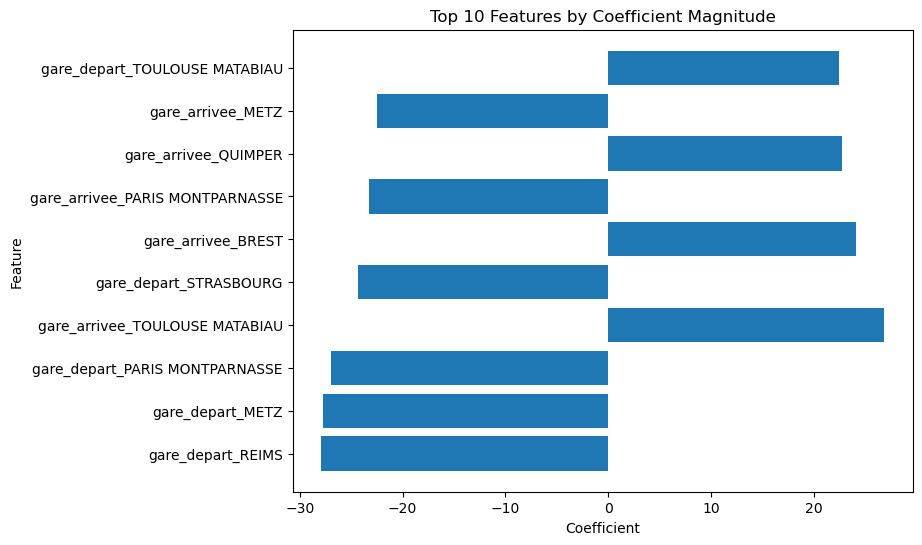
\includegraphics[width=12cm]{important_coefs.png}
\end{center}

\begin{center}
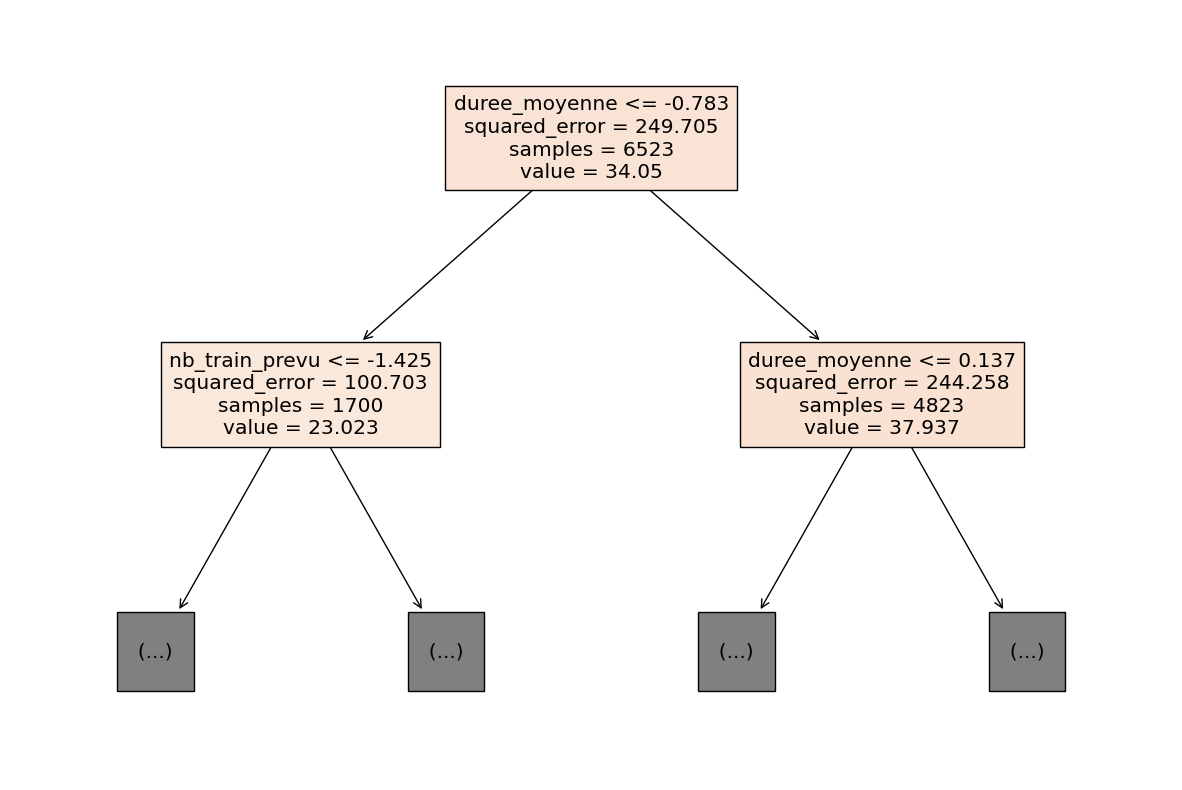
\includegraphics[width=12cm]{decision_tree.png}
\end{center}
Pour les poids de la régression linéaire, on voit que ce sont des gares issues du one hot encoding qui sont les plus importantes. Par exemple, le départ / l'arrivée de / à Toulouse Matabiau a fortement tendance à augmenter le retard.
Pour l'arbre de décision, c'est la durée moyenne et le nombre de trains qui paraissent être les features les plus importantes.

\section{Sélection de modèles}
Nous avons testé différents modèles pour ce problème de régression :
\begin{itemize}[label=\textbullet]
    \item Régression linéaire
    \item Régression linéaire avec régularisation Ridge
    \item Régression linéaire avec régularisation Lasso
    \item k Nearest Neighbors (kNN)
    \item Support Vector Machine (SVM)
    \item Arbre de décision
    \item Random Forest
    \item Extremely randomized trees
    \item AdaBoost
    \item Extreme Gradient Boosting
\end{itemize}

\subsection{Grid Search}
Pour sélectionner les modèles en testant différentes combinaisons d'hyperparamètres, nous avons utilisé une méthode de Grid Search avec cross-validation. Nous évaluons les modèles avec leur $R^2$ et leur RMSE (Root Mean Squared Error) sur un ensemble de test séparé des données d'entraînement. Voici les résultats dans un tableau ainsi que sous forme de nuage de points.

\begin{center}
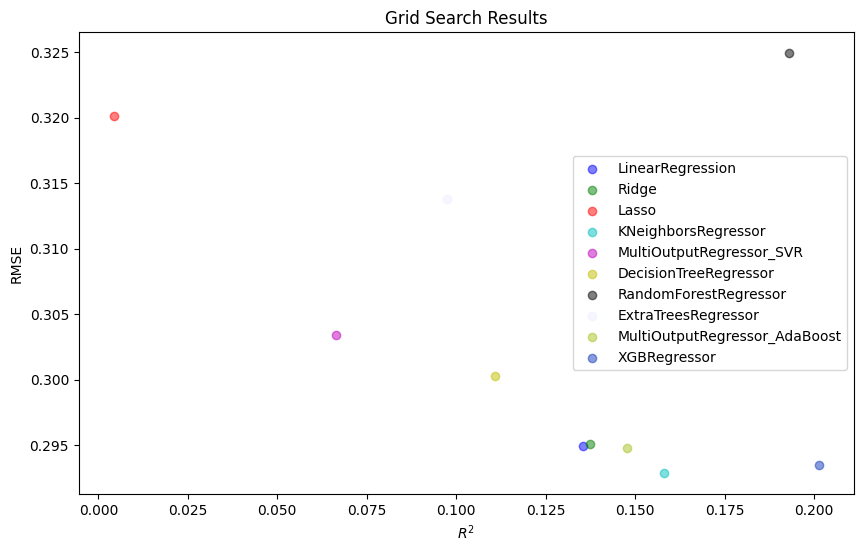
\includegraphics[width=12cm]{grid_search_results.png}
\end{center}

\begin{center}
\begin{tabular}{lcc}
\textbf{Model} & \textbf{$R^2$} & \textbf{RMSE} & \textit{Best parameters} \\[1mm] \hline \\[-2mm]
LinearRegression & 0.135 & 0.295 & \textit{{'fit\_intercept': True}} \\[1mm] \hline \\[-1.3mm]
Ridge & 0.138 & 0.295 & \textit{{'alpha': 1.0}} \\[1mm] \hline \\[-1.3mm]
Lasso & 0.004 & 0.320 & \textit{{'alpha': 0.1}} \\[1mm] \hline \\[-1.3mm]
KNeighborsRegressor & 0.158 & 0.293 & \textit{{'n\_neighbors': 76, 'weights': 'distance'}} \\[1mm] \hline \\[-1.3mm]
MultiOutputRegressor\_SVR & 0.066 & 0.303 & \textit{{'estimator\_\_C': 0.1, 'estimator\_\_kernel': 'linear'}} \\[1mm] \hline \\[-1.3mm]
DecisionTreeRegressor & 0.111 & 0.300 & \textit{{'max\_depth': 60, 'min\_samples\_leaf': 40, 'min\_samples\_split': 2}} \\[1mm] \hline \\[-1.3mm]
RandomForestRegressor & 0.193 & 0.325 & \textit{{'n\_estimators': 200, 'max\_depth': 50}} \\[1mm] \hline \\[-1.3mm]
ExtraTreesRegressor & 0.097 & 0.314 & \textit{{'n\_estimators': 200, 'max\_depth': 10}} \\[1mm] \hline \\[-1.3mm]
MultiOutputRegressor\_AdaBoost & 0.148 & 0.295 & \textit{{'estimator\_\_n\_estimators': 10, 'estimator\_\_learning\_rate': 0.01}} \\[1mm] \hline \\[-1.3mm]
XGBRegressor & 0.201 & 0.293 & \textit{{'n\_estimators': 100, 'learning\_rate': 0.1, 'max\_depth': 3}} \\ \\ \hline
\end{tabular}
\end{center}

\bigskip
On remarque d'abord que tous les modèles ont des $R^2$ très faibles (maximum autour de 0.2), ce qui veut dire que nos modèles n'arrivent globalement pas à expliquer la variance de nos variables cibles. Nos variables explicatives ne sont donc sûrement pas suffisantes pour prédire correctement nos variables cibles.

Parmi les modèles testés, les meilleurs sont le XGBRegressor, le kNN, Adaboost, et la régression linéaire (avec ou sans Ridge). Le XGBRegressor atteint le meilleur $R^2$, mais a une RMSE équivalente au kNN et même à la régression linéaire. En tenant compte de l'argument qu'un modèle simple généralisera mieux qu'un modèle plus complexe en temps général, la régression linéaire pourrait être choisie comme meilleur modèle ici.




\section{Ouverture : émissions CO2}
Les émissions CO2 sont rarement un facteur pris en compte lors de la mise en place de solution de Machine Learning, alors que c'est un facteur important dans le contexte actuel. Voici donc un aperçu des émissions de CO2 enregistrées pour nos modèles les plus performants en terme d'erreur :

\begin{center}
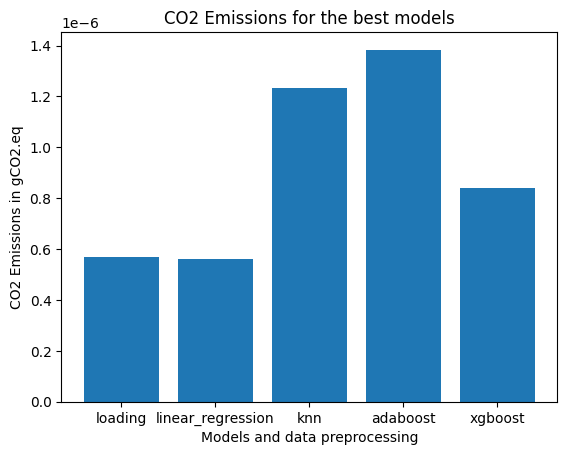
\includegraphics[width=15cm]{CO2_emissions.png}
\end{center}

Cela permet d'avoir un 2ème critère de choix pour choisir le modèle. "loading" correspond aux ressources nécessaires pour charger les données et les transformer à travers toute la pipeline de preprocessing. C'est plus de ressources que pour entraîner et effectuer une prédiction sur l'ensemble de test pour la régression linéaire.
Ici, on choisirait donc plutôt une régression linéaire car elle consomme moins de ressources pour être entraînée et faire la prédiction que les autres modèles, pour une performance équivalente. On s'y attendait car c'est un modèle très simple. Dans le cas où aucun modèle simple ne rivalise avec des modèles plus complexes, il peut être intéressant de voir si un compromis entre performance et ressources nécessaires est possible.

\end{document}
